\lstset{style=Python,basicstyle=\ttfamily\tiny}

\fboxsep=.6pt

% Default settings for listings
\lstset{style=python}

\title[Grundlagenfach]{Informatik, Grundlagenfach}
\subtitle{Semesterprogramm \& Einführung (FDU)}

\author[Blum, Cyril]{Cyril Blum}

\institute[FDU]
{
    Fachschaft Informatik\\
    Kantonsschule Stadelhofen -- Filiale Dübendorf (FDU)
}

\date[\today]

\titlegraphic{\vspace{-.3cm}\includegraphics[height=1.8cm,keepaspectratio]{"Grundlagen_Info/06_Datenbanken/Figures/title-emojis"}}

\frame{\titlepage}

\begin{frame}\sectionframe[FDUblue]{Einleitung}{Willkommen im Grundlagenfach Informatik}
\end{frame}

\begin{frame}{Einleitung}
    \begin{itemize}[<+->]
        \item[\faCheckSquare] Themenübersicht
        \item[\faCheckSquare] Geschichte der Informatik
        \item[\faCheckSquare] Lernziele
        \item[\faCheckSquare] Semesterplan
        \item[\faCheckSquare] Prüfungsdaten \& Regeln
        \item[\faCheckSquare] Vorstellung
        \item[\faCheckSquare] Grundwerte \& Regeln
        \item[\faCheckSquare] Benotung
        \item[\faCheckSquare] Fragen
    \end{itemize}
\end{frame}

\begin{frame}\sectionframe[FDUteal]{Geschichte der Informatik}{Köpfe, die unser Fach geprägt haben}
\end{frame}

\begin{frame}{Geschichte: Theorie \& Computer-Pioniere}
    \begin{columns}[c]
        \begin{column}{0.33\textwidth}
            \centering
            \IfFileExists{Customizations/FDU/assets/people/lovelace.jpg}{%
                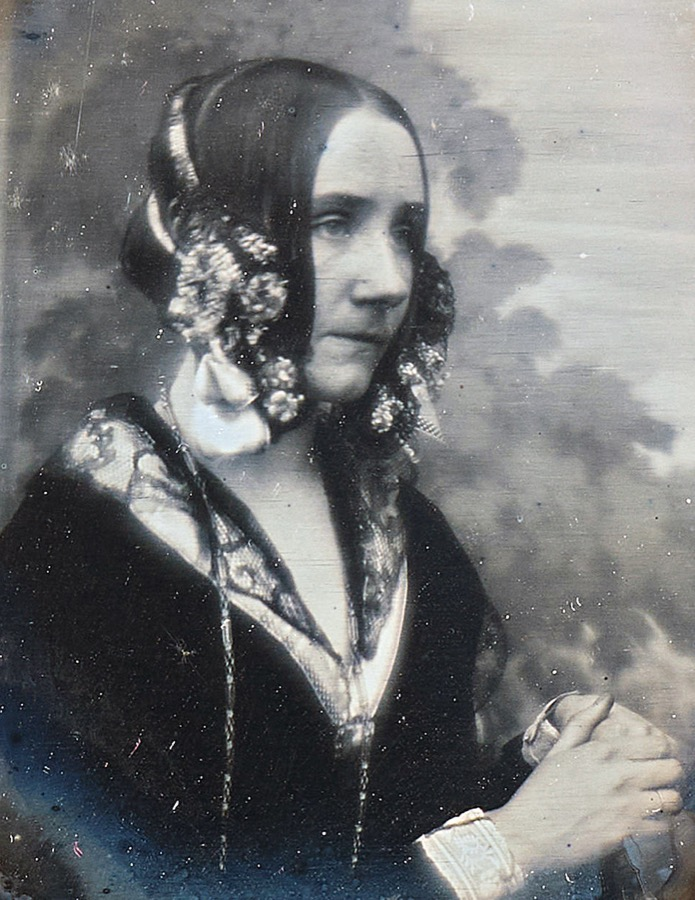
\includegraphics[height=2.7cm,keepaspectratio]{Customizations/FDU/assets/people/lovelace.jpg}%
            }{}\\[1mm]
            \textbf{\color{FDUteal}Ada Lovelace}\\
            {\tiny 1815\,--\,1852, England}\\[1mm]
            \footnotesize Erster veröffentlichter \textbf{Algorithmus} (1843). Gilt als erste Programmiererin.
        \end{column}
        \begin{column}{0.33\textwidth}
            \centering
            \IfFileExists{Customizations/FDU/assets/people/turing.jpg}{%
                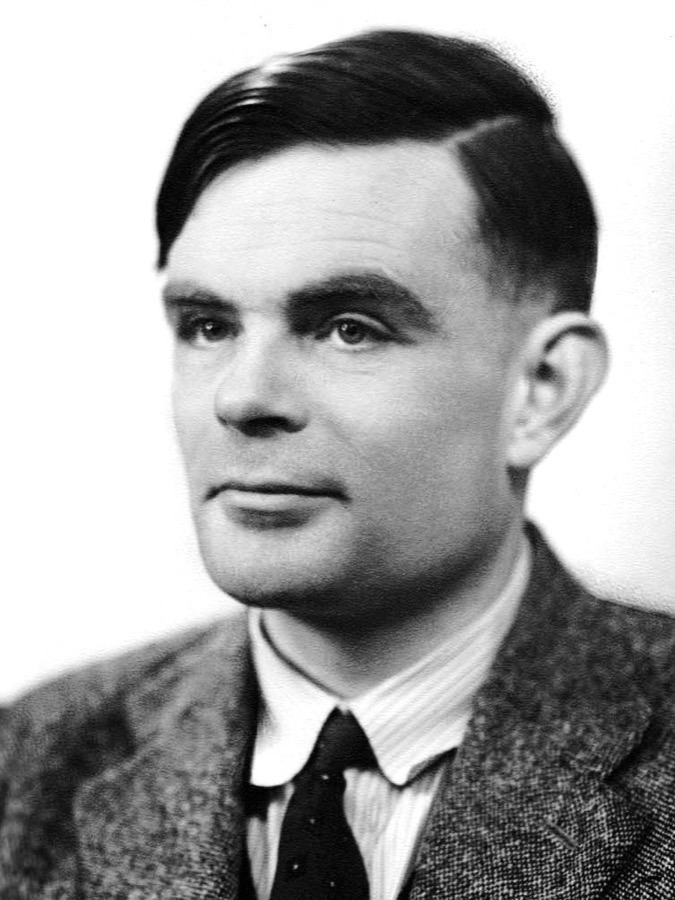
\includegraphics[height=2.7cm,keepaspectratio]{Customizations/FDU/assets/people/turing.jpg}%
            }{}\\[1mm]
            \textbf{\color{FDUteal}Alan Turing}\\
            {\tiny 1912\,--\,1954, England}\\[1mm]
            \footnotesize Erfand die \textbf{Turingmaschine} (theoretischer Computer) \& knickte Enigma.
        \end{column}
        \begin{column}{0.33\textwidth}
            \centering
            \IfFileExists{Customizations/FDU/assets/people/zuse.jpg}{%
                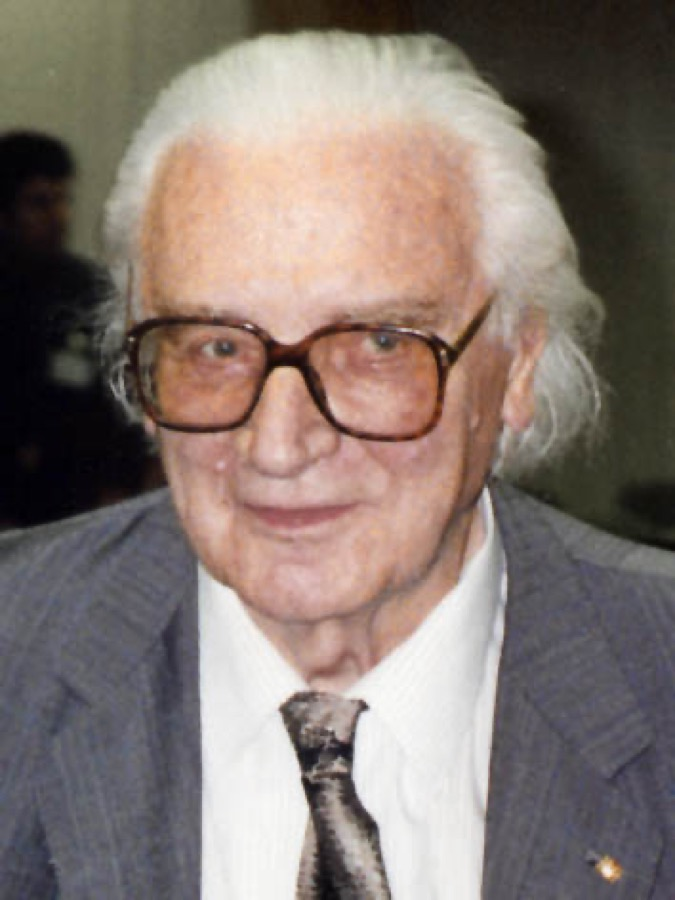
\includegraphics[height=2.7cm,keepaspectratio]{Customizations/FDU/assets/people/zuse.jpg}%
            }{}\\[1mm]
            \textbf{\color{FDUteal}Konrad Zuse}\\
            {\tiny 1910\,--\,1995, Deutschland}\\[1mm]
            \footnotesize Baute 1941 den \textbf{Z3} -- den 1. programmierbaren binären Computer.
        \end{column}
    \end{columns}
\end{frame}

\begin{frame}{Geschichte: Schaltungen \& Software-Meilensteine}
    \begin{columns}[c]
        \begin{column}{0.33\textwidth}
            \centering
            \IfFileExists{Customizations/FDU/assets/people/babbage.jpg}{%
                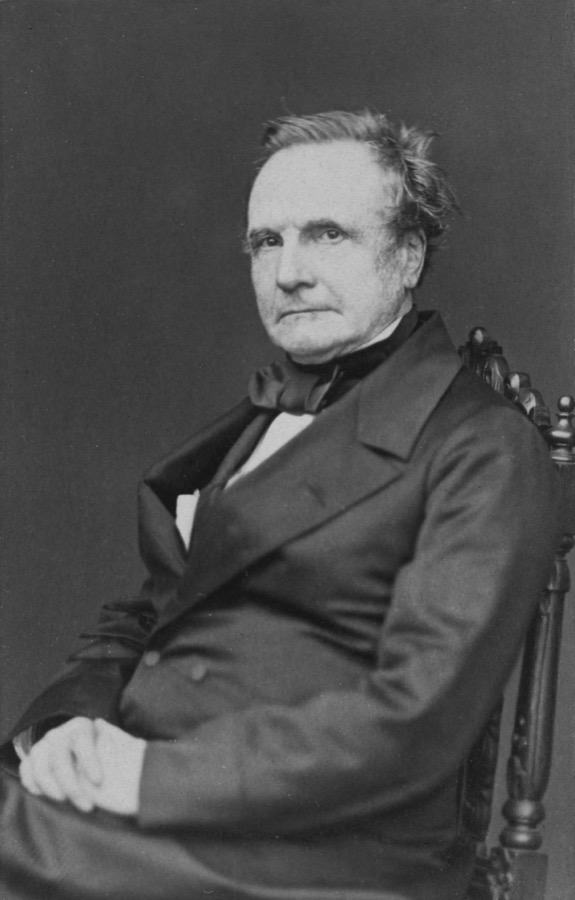
\includegraphics[height=2.7cm,keepaspectratio]{Customizations/FDU/assets/people/babbage.jpg}%
            }{}\\[1mm]
            \textbf{\color{FDUteal}Charles Babbage}\\
            {\tiny 1791\,--\,1871, England}\\[1mm]
            \footnotesize Entwarf die \textbf{Analytical Engine} -- Vorläufer mechanischer Computer.
        \end{column}
        \begin{column}{0.33\textwidth}
            \centering
            \IfFileExists{Customizations/FDU/assets/people/shannon.jpg}{%
                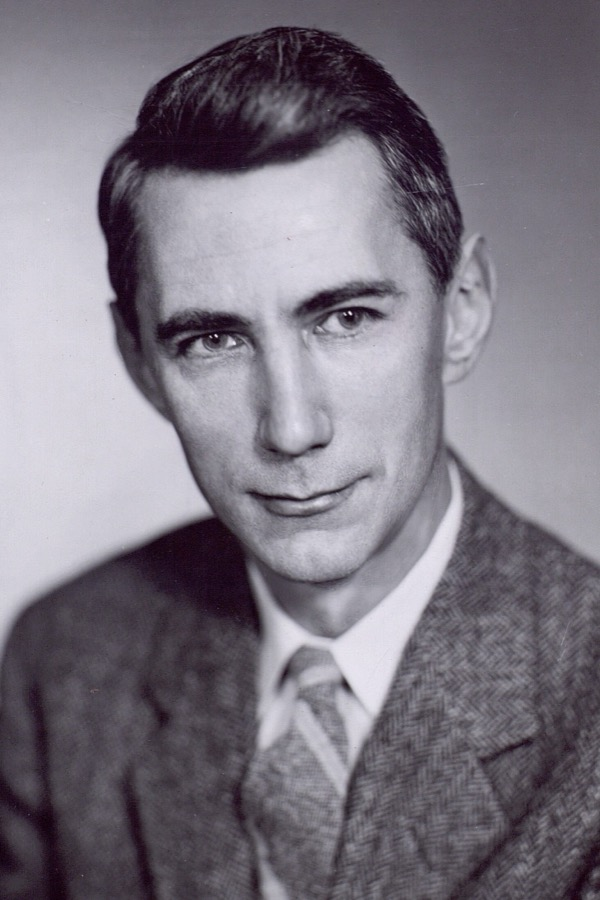
\includegraphics[height=2.7cm,keepaspectratio]{Customizations/FDU/assets/people/shannon.jpg}%
            }{}\\[1mm]
            \textbf{\color{FDUteal}Claude Shannon}\\
            {\tiny 1916\,--\,2001, USA}\\[1mm]
            \footnotesize Verknüpfte Logik mit Schaltungen (1937) \& erfand den Begriff \textbf{Bit}.
        \end{column}
        \begin{column}{0.33\textwidth}
            \centering
            \IfFileExists{Customizations/FDU/assets/people/hopper.jpg}{%
                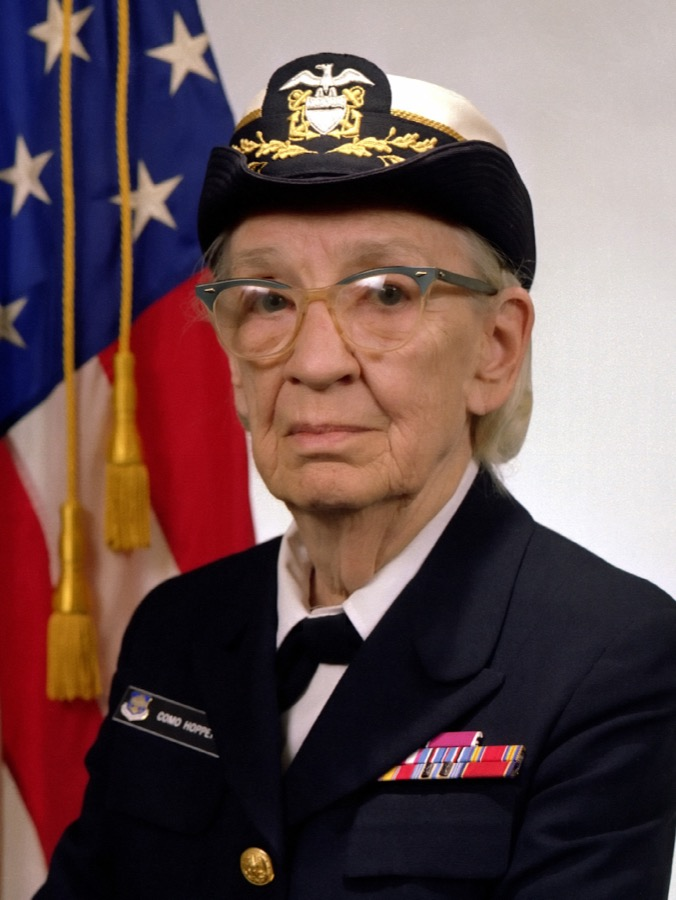
\includegraphics[height=2.7cm,keepaspectratio]{Customizations/FDU/assets/people/hopper.jpg}%
            }{}\\[1mm]
            \textbf{\color{FDUteal}Grace Hopper}\\
            {\tiny 1906\,--\,1992, USA}\\[1mm]
            \footnotesize Erster \textbf{Compiler} (menschenlesbarer Code) \& der 1. \textbf{Bug} (Motte).
        \end{column}
    \end{columns}
\end{frame}

\begin{frame}\sectionframe[FDUteal]{Themenübersicht}{Was erwartet Sie im Grundlagenfach?}
\end{frame}

\begin{frame}[fragile]{Themenübersicht}{Programmieren}
    \begin{center}
        \begin{minipage}{.4\textwidth}
            \begin{lstlisting}[escapechar=!]
import turtle as t

for _ in range(10):   
    for _ in range(4):
        t.fd(100)
        t.rt(360 / 4) 
    t.rt(360 / 10)
    
t.done()
\end{lstlisting}
        \end{minipage}\hfill\begin{minipage}{.4\textwidth}
            \begin{figure}[H]
                \centering
                
\includegraphics[height=3.0cm,keepaspectratio]{Grundlagen_Info/00_Programmieren/Figures/viereck_blume}
            \end{figure}
        \end{minipage}
    \end{center}
    \only<2->{
    \begin{center}
        \textit{Program or be programmed} $\rightarrow$ nicht nur Apps konsumieren, sondern sich seine eigene Welt gestalten!
    \end{center}}
    \only<3->{
    \begin{center}
        \textit{Was würden Sie gerne selbst programmieren?}
    \end{center}}
\end{frame}

\begin{frame}[fragile]{Themenübersicht}{Programmieren}
    \begin{columns}[c]
        \begin{column}{0.62\textwidth}
            \begin{figure}[H]
                \centering
                \includegraphics[height=2.3cm,keepaspectratio]{Grundlagen_Info/00_Programmieren/Figures/Glattalbahn_vbg}
            \end{figure}
            \begin{lstlisting}
stationen = ["Sternen", "Messe", "Leutschenbach", "Oerlikerhus", "Glattpark", "Lindbergh", "Glattbrugg", "Bäuler", "Unterriet", "Kloten", "Flughafen", "Flughafen Fracht"]
dauer = [0, 60, 122, 185, 241, 363, 543, 603, 666, 729, 786, 845]
\end{lstlisting}
        \end{column}
        \begin{column}{0.05\textwidth}
            $\Rightarrow$
        \end{column}
        \begin{column}{0.30\textwidth}
            \begin{figure}[H]
                \centering
                \includegraphics[height=2.3cm,keepaspectratio]{Grundlagen_Info/00_Programmieren/Figures/tram-sbb.jpeg}
            \end{figure}
        \end{column}
    \end{columns}
\end{frame}

\begin{frame}[fragile]{Themenübersicht}{Kodierungen}
    \begin{center}
        \small\textit{Ohne Kodierungen gäbe es keine Emojis, TikToks oder YouTube.} $\rightarrow$ Wo begegnen Ihnen Kodierungen im Alltag?
    \end{center}
    \vspace{-2mm}
    \begin{figure}[H]
        \centering
        \begin{subfigure}{.48\textwidth}
            \centering
            \includegraphics[height=2.2cm,keepaspectratio]{Grundlagen_Info/13_ZahlendarstellungenUndKodierungen/Figures/rgb-farbmischung-1}
        \end{subfigure}
        \begin{subfigure}{.48\textwidth}
            \centering
            \includegraphics[height=2.2cm,keepaspectratio]{Grundlagen_Info/13_ZahlendarstellungenUndKodierungen/Figures/rgb-farbmischung-2}
        \end{subfigure}
    \end{figure}
    \vspace{-2mm}
    \centering\small $\rightarrow$ Jede Farbe kodiert zwischen 0 und 255!\\
    \only<2->{\footnotesize
        \red{11111111}\green{00000000}\blue{00000000} = \#\red{FF}\green{00}\blue{00} = \red{255}, \green{0}, \blue{0} = reines Rot\\
        \red{10000000}\green{10000000}\blue{10000000} = \#\red{80}\green{80}\blue{80} = \red{128}, \green{128}, \blue{128} = grau}
\end{frame}

\begin{frame}{Farben}{Themenübersicht}{Kodierungen}
    \begin{figure}[H]
        \centering
        \includegraphics[height=4.5cm,keepaspectratio]{Grundlagen_Info/13_ZahlendarstellungenUndKodierungen/Figures/colordepth}
    \end{figure}
\end{frame}

\begin{frame}{Themenübersicht}{Kodierungen}
    \begin{table}[H]
        \tiny
        \centering
        \begin{tabular}{@{}l|rr|l@{}}
            \toprule
            \textbf{Masseinheit} & \multicolumn{2}{l|}{\textbf{Dezimalsystem}} & Grössenordnung \\ \midrule
            KB (Kilobyte) & $10^3$ B(yte) & \num{1000} B & eine Text-Datei \\
            MB (Megabyte) & $10^6$ B & \num{1000000} B & eine Musik-Datei \\
            GB (Gigabyte) & $10^9$ B & \num{1000000000} B & eine Video-Datei \\
            TB (Terabyte) & $10^{12}$ B & \num{1000000000000} B & kleiner Firmen-Server \\
            PB (Petabyte) & $10^{15}$ B & ... & Facebook-Server \\
            EB (Exabyte) & $10^{18}$ B & ... & alle CERN-Daten \\
            ZB (Zettabyte) & $10^{21}$ B & ... & alle Daten ($\sim$ 100 ZB) \\
            YB (Yottabyte) & $10^{24}$ B & ... & $\sim$ 2030? \\ \bottomrule
        \end{tabular}
        \caption*{Gängige Daten-Grössenordnungen in der Informatik}
    \end{table}
    \only<2->{
        \begin{center}\small
            Wie nennt man ein \enquote{Megagramm} geläufiger?
        \end{center}}
\end{frame}

\begin{frame}[label=schemakrypto]{Themenübersicht}{Kryptologie}
    \begin{figure}[H]
        \centering
        \IfFileExists{Grundlagen_Info/03_Kryptologie/Figures/filius-annotated.png}{%
            \includegraphics[height=3.0cm,keepaspectratio]{Grundlagen_Info/03_Kryptologie/Figures/filius-annotated}%
        }{%
            \IfFileExists{Grundlagen_Info/07_Netzwerke/Figures/Wireshark Chat unencrypted Network.png}{%
                \includegraphics[height=3.0cm,keepaspectratio]{Grundlagen_Info/07_Netzwerke/Figures/Wireshark Chat unencrypted Network}%
            }{}%
        }%
        \begin{center}\small
            \only<1>{Was machen Sie alles im Internet?}
            \only<2>{
                \normalsize Z.B.: Sie schreiben eine Nachricht an Ihr \emoji{two-hearts}...\\
                ...und ich kann alles mitlesen! \emoji{teacher}}
        \end{center}
    \end{figure}
    \begin{center}\small
        Wer von Ihnen würde mir Zugriff auf all Ihre Chats, Daten und Fotos gewähren?
    \end{center}
\end{frame}

\begin{frame}{Themenübersicht}{Datenintegrität}
    \begin{center}
        \includegraphics[height=3.2cm,keepaspectratio]{Grundlagen_Info/05_Datenintegritaet/Figures/bitrot.png}
    \end{center}
    \begin{center}\small
        Haben Sie schon mal einen Datenfehler bemerkt?
    \end{center}
\end{frame}

\begin{frame}{Themenübersicht}{Datenintegrität}
    \begin{center}
        \includegraphics[height=3.8cm,keepaspectratio]{Grundlagen_Info/05_Datenintegritaet/Figures/NAS.png}
    \end{center}
\end{frame}

\begin{frame}{Themenübersicht}{Netzwerke}
    \begin{figure}[H]
        \centering
        \includegraphics[height=3.6cm,keepaspectratio]{Grundlagen_Info/07_Netzwerke/Figures/arpanet.png}
    \end{figure}
\end{frame}

\begin{frame}{Themenübersicht}{Netzwerke}
    \begin{figure}[H]
        \centering
        \includegraphics[height=3.6cm,keepaspectratio]{Grundlagen_Info/07_Netzwerke/Figures/internet_use_map_2024}
    \end{figure}
\end{frame}

\begin{frame}{Themenübersicht}{Netzwerke}
    \begin{figure}[H]
        \centering
        \includegraphics[height=3.6cm,keepaspectratio]{Grundlagen_Info/07_Netzwerke/Figures/subnets}
    \end{figure}
\end{frame}

\begin{frame}{Themenübersicht}{AI und Machine Learning}
    \begin{columns}[c]
        \begin{column}{0.48\textwidth}
        \small
        \begin{itemize}
            \item Beispiel: Note über Lernaufwand und Schlaf
            \item Erklärung:
                  \begin{itemize}
                      \item $x_1$: Lernaufwand
                      \item $x_2$: Schlaf
                      \item $y$: Note
                  \end{itemize}
        \end{itemize}
        \begin{block}{Formeln}
            \footnotesize
            \begin{itemize}[<+->]
                \item Einfache lineare Regression:
                      \[y = \textcolor{red}{a_0} + \textcolor{blue}{a_1} x_1\]
                \item Multiple lineare Regression:
                      \[y = \textcolor{red}{a_0} + \textcolor{blue}{a_1} x_1 + a_2x_2 + \cdots + a_n x_n\]
            \end{itemize}
        \end{block}
        \end{column}
        \begin{column}{0.50\textwidth}
        \begin{figure}[H]
            \centering
            \includegraphics[height=2.7cm,keepaspectratio]{Grundlagen_Info/10_KI_und_Algorithmen/Figures/linreg_3d.pdf}
        \end{figure}
        \end{column}
    \end{columns}
\end{frame}

\begin{frame}{Themenübersicht}{AI und Machine Learning}
    \begin{figure}[H]
        \centering
        \begin{tikzpicture}[scale=0.7, transform shape, ->, >=stealth', node distance=3.8cm, thick,
                website/.style={rectangle, draw, minimum width=2.2cm, minimum height=0.9cm, align=center}]

            \node[website] (moodle) {\texttt{moodle.ch}};
            \node[website] (intranet) [right of=moodle] {\texttt{intranet.kzn.ch}};
            \node[website] (yt) [below of=intranet] {\texttt{youtube.com}};
            \node[website] (20min) [below of=moodle] {\texttt{20minuten.ch}};

            \onslide<2>{
                \path[->]
                (moodle) edge[bend left] node[above] {0.9 (=90 \%)} (intranet)
                (moodle) edge[bend right=15] node[left] {0.1 (=10 \%)} (yt);
            }

            \onslide<3->{
                \path[->]
                (moodle) edge[bend left] node[above] {0.9} (intranet)
                (moodle) edge[bend right=15] node[left] {0.1} (yt);
            }
            \onslide<4->{
                \path[->]
                (intranet) edge[bend left] node[below] {0.8} (moodle)
                (intranet) edge node[right] {0.2} (yt);
            }
            \onslide<5->{
                \path[->] (yt.west) edge[bend left] node[below] {1} (20min.east);
            }
            \onslide<6->{
                \path[->]
                (20min.east) edge[bend left] node[above] {0.6} (yt.west)
                (20min) edge node[left] {0.4} (moodle);
            }
        \end{tikzpicture}
    \end{figure}
    \onslide<6->{
        \begin{center}\small
            Wenn Sie jetzt auf \texttt{moodle.ch} sind, welche Webseite möchten Sie am wahrscheinlichsten als nächstes besuchen?
        \end{center}
    }
\end{frame}

\begin{frame}{Lernziele}
    Am Ende des Grundlagenfachs Informatik können Sie:
    \small
    \begin{itemize}[<+->]
        \item[\faCheckSquare] Komplexe Programme in \textbf{Python} schreiben
        \item[\faCheckSquare] \textbf{Daten kodieren} und effiziente \textbf{Algorithmen} zur Datenanalyse entwickeln
        \item[\faCheckSquare] Erklären, wie \textbf{Computer und Netzwerke} funktionieren
        \item[\faCheckSquare] Daten sicher \textbf{verschlüsseln} und übertragen
        \item[\faCheckSquare] Die Grundlagen von \textbf{Künstlicher Intelligenz} und \textbf{Machine Learning} verstehen
        \item[\faCheckSquare] Die \textbf{gesellschaftlichen Auswirkungen} der Informatik einschätzen
        \item[\faCheckSquare] \textbf{Eigene Ideen} in Informatik-Projekten umsetzen
        \item[\faCheckSquare] \textcolor{FDUblue}{\textbf{Mit Freude Ihren Computer nutzen, um eigene Ideen umzusetzen!}}
    \end{itemize}
\end{frame}

\begin{frame}\sectionframe[FDUblue]{Semesterplan}{Ablauf \& Daten}
\end{frame}

\begin{frame}{Semesterplan}
    \begin{center}
        \faFileExcel{} \textbf{Semesterplan} (provisorisch)
    \end{center}
\end{frame}

\begin{frame}\sectionframe[FDUteal]{Prüfungsdaten}{Leistungsnachweise \& Richtlinien}
\end{frame}

\begin{frame}{Prüfungsdaten}{Leistungsnachweise}
    \begin{block}{\faFileExcel{} Bereitstellung der Prüfungsdaten}
        Die Übersicht aller Prüfungstermine steht Ihnen ab \textbf{nächster Woche als Excel-Datei} im Teams-Kanal der Klasse zur Verfügung (nur Leserechte).
    \end{block}
    
    \vspace{2mm}
    \begin{itemize}[<+->]
        \item[\faCalendarCheck] \textbf{Transparenz}: Alle Prüfungen aller Fächer sind in einer zentralen Übersicht erfasst.
        \item[\faExclamationTriangle] \textbf{Maximal-Belastung}: 
            \begin{itemize}
                \item Max. \textbf{3 grosse Leistungsnachweise} pro Woche
                \item Max. \textbf{1 grosser Leistungsnachweis} pro Tag
            \end{itemize}
        \item[\faBullhorn] \textbf{Information}: Lehrpersonen informieren Sie im Fachunterricht zusätzlich direkt über Ihre jeweiligen Prüfungstermine.
    \end{itemize}
\end{frame}

\begin{frame}{Prüfungsdaten}{Schulisches Vorgehen für Lehrpersonen \& Klassen}
    \small
    \begin{enumerate}[<+->]\setlength{\itemsep}{1pt}
        \item \textbf{Ablage im Teams}: Klassenlehrperson legt Klassendatei im Lehrpersonenteams ab.
        \item \textbf{Eintragung}: Lehrpersonen tragen Leistungsnachweise ein (Max. 3/Woche, Max. 1/Tag). Erster Eintrag gewährt keinen Vorrang bei Kollisionen.
        \item \textbf{Frist}: Eintragung aller Termine bis spätestens Montag der 1. Schulwoche.
        \item \textbf{Bereinigung}: Klassenlehrperson prüft Häufungen und koordiniert Lösungen.
        \item \textbf{Freigabe}: Tabelle wird spätestens am \textbf{Montag der 2. Schulwoche} für Schüler/-innen freigegeben (Leserechte).
        \item \textbf{Verschiebungen}: Werden später Prüfungen verschoben oder ergänzt, muss die Max.-Regel (3/Woche, 1/Tag) weiterhin eingehalten werden.
    \end{enumerate}
\end{frame}

\begin{frame}\sectionframe[FDUblue]{Vorstellung}{Lernen wir uns kennen}
\end{frame}

\begin{frame}{Vorstellung}
\centering
\scalebox{0.78}{%
\begin{tikzpicture}[m/.style={draw, color=FDUblue, text=black, align=left, font=\tiny, fill=FDUblue!30, fill opacity=.3, rounded corners,text opacity=1}]
    \node[anchor=south west,inner sep=0] at (0,0) {\includegraphics[width=\textwidth]{"Private/Presentation/ch"}};
    
    % Burgdorf
    \node[m](Burgdorf) at (5.8,5.1) {\faMapMarker{} Burgdorf};
    
    \only<2->{
	    % Bern
        \node[m](Bern) at (5.0,4.7) {\faMapMarker{} Bern\\\includegraphics[width=1cm]{"Private/Presentation/Logos/logo_gk"}};
        \draw (Burgdorf.north) edge[->, bend right=90] (Bern.north);}
    
    \only<3->{
	    % Fribourg
        \node[m](Fribourg) at (4.2,3.9) {\faMapMarker{} Fribourg\\\includegraphics[width=.7cm]{"Private/Presentation/Logos/logo unifr"}};
        \draw (Bern.south) edge[->, bend left=30] (Fribourg.east);
    }
    
    \only<4->{
    	% Lausanne
        \node[m](Lausanne) at (2.6,3.1) {\faMapMarker{} Lausanne\\\includegraphics[width=.7cm]{"Private/Presentation/Logos/logo epfl"}};
       	\draw (Fribourg.south) edge[->, bend left=30] (Lausanne.east);
    }  
    
    \only<5->{
        % Netherlands
        \node[m](Wageningen) at (1.5,7.8) {\faMapMarker{} Wageningen\\\includegraphics[width=1.3cm]{"Private/Presentation/Logos/logo_wur"}};    
        \draw[dashed] (Lausanne.north) edge[->, bend left=15] (Wageningen.south);
        \draw[dashed] (Wageningen.south) edge[->, bend left=15] (Lausanne.north);
    }

	\only<6->{
	    % Paris
        \node[m](Paris) at (0.0,6.0) {\faMapMarker{} Paris\\\includegraphics[width=.9cm]{"Private/Presentation/Logos/logo_cdi"}};
        \draw (Lausanne.west) edge[->, bend left=15] (Paris.south);
    }
    
	\only<7->{
	    % Zürich
        \node[m](Zurich) at (6.6,5.6) {\faMapMarker{} Zürich\\\includegraphics[width=.7cm]{"Private/Presentation/Logos/PartnerRe"}};
        \draw (Paris.east) edge[->, bend left=15] (Zurich.west);
    }
    
    \only<8->{
   		% Dübendorf (FDU)
     	\node[m](Duebendorf) at (8.3,6.9) {\faMapMarker{} Dübendorf (FDU)\\
\includegraphics[height=4.5mm]{Customizations/FDU/assets/02_System_Stempelversion_Logo_RZ_schwarz.pdf}};
	     \draw (Zurich.east) edge[->, bend left=25] (Duebendorf.west);  
    }
\end{tikzpicture}%
}
\end{frame}

\begin{frame}{Interessen}
\begin{center}
\href{https://cblum.ch}{cblum.ch}
\end{center}
\end{frame}

\begin{frame}{Hauptziel}
\begin{center}
    \only<1>{\textcolor{FDUblue}{\faGraduationCap \textbf{Abschluss:} Maturität}}
    \only<2->{\sout{\textit{\textcolor{FDUblue}{\faGraduationCap \textbf{Abschluss:} Maturität}}}\\
    \vspace{4mm}
    \textcolor{FDUteal}{\Large\textbf{Spass an der Informatik und am eigenen Computer gewinnen!}}}
\end{center}
\end{frame}

\begin{frame}\sectionframe[FDUteal]{Grundwerte \& Regeln}{Für ein erfolgreiches Schuljahr}
\end{frame}

\begin{frame}{Grundwerte \& Regeln}
    \begin{overviewBox}
        \textit{Achte auf Deine Gedanken, denn es liegt in der Natur des Gedankes, Wirklichkeit zu werden.}
    \end{overviewBox}
    \begin{itemize}[<+->]
        \item[\faShoppingBag] Nutzen Sie Ihre wertvolle Zeit $\rightarrow$ Füllen Sie Ihren Rucksack
        \item[\faComments] Seien Sie \textbf{proaktiv}, fragen Sie nach
        \item[\faExclamationTriangle] Machen Sie \textbf{Fehler}, probieren Sie Dinge aus!
        \item[\faThumbsUp] Geben Sie mir \textbf{konstruktives Feedback}
    \end{itemize}
\end{frame}

\begin{frame}{Grundwerte \& Regeln}
    \begin{enumerate}
        \item Dokument (Semesterplanung) bitte durchlesen
        \item Änderungen und Erweiterungen vorschlagen
        \item Dokument vorne unterschreiben
    \end{enumerate}
    Vielen Dank!
\end{frame}

\begin{frame}\sectionframe[FDUblue]{Benotung}{Richtlinien für die Bewertung}
\end{frame}

\begin{frame}{Benotung}
    \begin{enumerate}[<+->]
        \item[\faPen] Jede \textbf{schriftliche Prüfung} zählt 1 Note
        \item[\faMoneyBill] \textbf{Boni}: Mündliche Beteiligung und Feedback an mich (kann nur positiv sein)
        \item[\faFilePdf] Richtlinien als PDF auf Teams/Moodle -- bitte lesen und Fragen stellen!
    \end{enumerate}
\end{frame}

\begin{frame}{\faQuestionCircle}\Huge
    \begin{center}
        Fragen?
    \end{center}
\end{frame}
